\documentclass[12pt,a4paper]{article}
\usepackage[utf8]{inputenc}
\usepackage[czech]{babel}
\usepackage[T1]{fontenc}
\setlength{\parskip}{12pt}
\usepackage{fullpage}
\usepackage{ amssymb }
\usepackage{ mathrsfs }
\usepackage{amsthm}
\usepackage{amsmath}
\usepackage{fixltx2e}
\newtheorem{definition}{Definice}
\newtheorem{sentence}{Věta}
\newtheorem{example}{Příklad}
\usepackage{graphicx}

\begin{document}

\title{Státnicový okruh 1: \\ Matematické metody}
\maketitle
\newpage
\tableofcontents
\newpage
\textbf{Množiny, operace s množinami, kartézský součin množin, konečné, spočetné a nespočetné množiny. Číselné
množiny. Princip indukce. Relace a jejich vlastnosti, operace s relacemi, reprezentace relací. Binární relace na
množině, uzávěry relací, ekvivalence, rozklad na množině, uspořádané množiny. Zobrazení a jejich vlastnosti.}

\section{Množiny}
Množina je objekt, který se skládá z jiných objektů tzv. \textbf{prvků} té množiny. Množiny zpravidla značíme velkými písmeny (A, B, \dots, Z), jejich prvky pak malými písmeny (a, b, \dots, z). Fakt, že $x$ je prvkem množiny $A$ značíme $x \in A$. Není-li prvkem $A$ značíme $x \not\in A$.

Množina je jednoznačné dána svými prvky. Prvek do množiny buď patní nebo ne. Nemá tedy smysl hovořit o pořadí prvků a také nemá smysl zabývat se tím kolikrát se daný prvek v množině nachází.
Speciální množinou je tzv. \textbf{prázdná množina} značíme $\emptyset$. Tato množina neobsahuje žádné prvky tedy pro všechna $x$ platí, že $x \not\in \emptyset$.

\subsection{Dělení množin}
Množiny dělíme na \textbf{konečné} a \textbf{nekonečné}. Množina $A$ se nazývá konečná právě když existuje přirozené číslo $n$ tak že prvky této množiny můžeme očíslovat čísly 1, 2, \dots, $n$. Číslo $n$ nazveme počet prvků množiny a značíme jej $|A|$
Pokud $|A| = \infty$ nazveme množinu nekonečnou a říkáme, že má nekonečně mnoho prvků.

\textbf{Spočetná} množina znamená zjednodušeně řečeno „množina, jejíž prvky lze spočítat“. Spočítáním se zde rozumí očíslování prvků množiny přirozenými čísly - přitom je jedno, zda použiji konečný nebo nekonečný počet přirozených čísel.

\subsection{Zapisování množin}
Množiny můžeme zapisovat následujícími způsoby:
\begin{enumerate}
	\item \textbf{Výčtem prvků} - Množinu která obsahuje prvky $a_1,a_2,\dots,a_n$ zapíšeme následovně $\{a_1,a_2,\dots,a_n\}$.
	\item \textbf{Pomocí charakteristické vlastnosti} - Množina obsahuje právě ty prvky, které splňují vlastnost $\varphi(x)$ zapisujeme $\{x | \varphi(x)\}$. Vlastnost $\varphi(x)$ může být popsána i slovně. Příklad $\varphi(x)$: číslo x je sudé.
\end{enumerate}
\subsection{Vztahy mezi množinami}
Základními vztahy mezi množinami jsou \textbf{rovnost} (=) a \textbf{inkluze} ($\subseteq$)
\begin{itemize}
	\item[] $A = B$ znamená, že pro každé $x : x \in A$ právě když $x \in B$
	\item[] $A \subseteq B$ znamená, že pro každé $x$ : jestliže $x \in A$ pak $x \in B$
	\item[] $A \not= B$ znamená že neplatí $A = B$
	\item[] $A \not\subseteq B$ znamená, že neplatí $A \subseteq B$
\end{itemize}

Množina jejichž prvky jsou právě všechny podmnožiny dané množiny $X$, nazýváme \textbf{potenční množina} množiny $X$ značí se $\mathscr{P}(X)$ nebo také $2^X$. Tedy $2^X = \{A|A\subseteq X\}$.

\subsection{Operace s množinami}
Mezi základní operace s množinami patří průnik (značí se $\cap$), sjednocení (značí se $\cup$), rozdíl (značí se $\setminus$).

Jsou-li $A,B$ množiny, definujeme množiny $A \cup B, A \cap B, A \setminus B$ následovně:
\begin{itemize}
	\item[] $A \cap B = \{ x|x \in A \text{ a } x \in B\}$ 
	\item[] $A \cup B = \{ x|x \in A \text{ nebo } x \in B\}$ 
	\item[] $A \setminus B = \{ x|x \in A \text{ a } x \not\in B\}$ 
\end{itemize}

Množiny nazýváme navzájem disjunktní právě když $A \cap B = \emptyset$.

\subsubsection{Vlastnosti operací}
\begin{itemize}
	\item $A \cap \emptyset = \emptyset, \hspace{10pt} A \cup \emptyset = A,\hspace{10pt} A \cap A = A$
	\item $A \cup B = B \cup A, \hspace{10pt} A \cap B = B \cap A$
	\item $(A \cup B) \cup C = A \cup (B \cup C)$
	\item $A \cap (B \cup C) = (A \cap B) \cup (A \cap C), \hspace{10pt} A \cup (B \cap C) = (A \cup B) \cap (A \cup C)$ 
	\item $A \cup (A \cap B) = A, \hspace{10pt} A \cap (A \cup B) = A$ 
\end{itemize}

\section{Relace}
Pojem relace je matematickým protějškem pojmu \textit{vztah}. Různé objekty jsou nebo nejsou v různých vztazích. Například číslo 3 je ve vztahu \uv{být menší} s číslem 5. Vztah je také určen aritou tj. počtem objektů které do vztahu vstupují, výše uvedený příklad má aritu 2 protože porovnáváme 2 čísla. Takovou relaci nazveme binární. Dále máme unární (jeden prvek), ternární (tři prvky), \dots

\begin{definition}
Kartézský součin množin $X_1, X_2, \dots,X_n$ je množina $X_1 \times X_2 \times \dots \times X_n$ definovaná předpisem $$X_1 \times \dots \times X_n =  \{\langle x_1, \dots x_n \rangle | x_1 \in X_1, \dots, x_n \in X_n\} $$
\end{definition}
 Kartézský součin $n$ množin je množina všech uspořádaných n-tic prvků z těchto množin. Je-li $X_1 = \dots = X_n = X$ pak $X_1 \times \dots \times X_n$ značíme také $X^n$ (n-tá kartézská mocnina množiny $X$)

\begin{definition}
Nechť $X_1, \dots,X_n$ jsou množiny. Relace mezi $X_1, \dots,X_n$ je libovolná podmnožina kartézského součinu $X_1 \times \dots \times X_n $.
\end{definition}

\begin{example}
Mějme množinu $A = \{1,2,3,4\}$ a množinu $B = \{a,b,c,d\}$. Relace $R,S \subseteq A \times B$ mohou vypadat následovně. $$R = \{\langle 1, a\rangle, \langle 1, b\rangle, \langle 3, d\rangle, \langle 4, a\rangle\}$$
$$S = \{\langle 3, a\rangle, \langle 1, c\rangle,  \langle 4, c\rangle\}\}$$
\end{example}

\subsection{Operace s (binárními) relacemi}
Relace jsou množiny n-tic. Proto s nimi jde provádět množinové operace ($\cap,\cup,\setminus$) a lze na ně aplikovat rovnost a inkluzi ($=, \subseteq$).
S binárními relacemi můžeme provádět další operace. Začněme tzv. inverzní relací k relaci $R \subseteq X \times Y$ je relace $R^{-1}$ definovaná předpisem: $$R^{-1} = \{\langle y, x \rangle | \langle x, y \rangle \in R\}$$
Další operací je tzv. skládání Je-li $R$ relací mezi množinami $X$ a $Y$ a $S$ relací mezi množinami $Y$ a $Z$, pak složením relací $R$ a $S$ je relace \( R \circ S \) mezi $X$ a $Z$ definovaná předpisem: $$R \circ S = \{\langle x, z \rangle | \exists y \in Y : \langle x,y\rangle \in R \text{ a } \langle y,z \rangle \in S\}$$

\begin{sentence}
	Pro relace $R \subseteq X \times Y, S \subseteq Y \times Z, T \subseteq Z \times U$ platí:
	\begin{itemize}
		\item[a)] $(R^{-1})^{-1} = R$
		\item[b)] $(R \circ S)^{-1} = S^{-1} \circ R^{-1}$
		\item[c)] $R \circ (S \circ T) = (R \circ S) \circ T$
	\end{itemize}
\end{sentence}

\subsection{Reprezentace relací}

\subsubsection{Tabulkou}
Binární relace lze znázorňovat tabulkami. Například relace \\$R = \{ \langle 1, \alpha \rangle, \langle 2, \gamma \rangle, \langle 1, \delta \rangle, \langle 2, \beta \rangle, \langle 3, \alpha \rangle\}$ mezi množinami \\$X = \{1,2,3\}$ a $Y = \{\alpha, \beta, \gamma, \delta, \epsilon\}$ je znázorněna následující tabulkou.

\begin{center}
	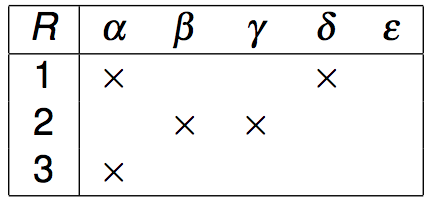
\includegraphics[scale=0.5]{images/1/RelationTable}
\end{center}

Tedy je-li $\langle x, y \rangle \in R$, je v průsečíku řádku $x$ a sloupce $y$ symbol $\times$, jinak tam není nic.

\subsubsection{Maticí}
Matice typu $m \times n$ je obdélníkové schéma o $m$ řádcích a $n$ sloupcích, ve kterém se na každém místě odpovídajícím nějakému řádku a nějakému sloupci nachází nějaká (nejčastěji číselná) hodnota. Označme tuto matici $M$, pro každé $i \in \{1, \dots,m\}$ a $j \in \{1,\dots,n\}$  Nechť $R$ je relace mezi množinami $X = \{x_1,\dots,x_m\}$ a $Y = \{y_1, \dots, y_n\}$. Potom relaci $R$ reprezentujeme maticí tak, že pokud:
$$\langle x_i,y_j\rangle \in R \text{ pak } m_{ij} = 1$$ 
$$\langle x_i,y_j\rangle \not\in R \text{ pak } m_{ij} = 0$$ 
Tuto matici nazveme \textbf{matice relace} R a značíme ji $M_R$. Matice $M_R$ relace $R = \{ \langle 1, \alpha \rangle, \langle 2, \gamma \rangle, \langle 1, \delta \rangle, \langle 2, \beta \rangle, \langle 3, \alpha \rangle\}$ mezi množinami \\$X = \{1,2,3\}$ a $Y = \{\alpha, \beta, \gamma, \delta, \epsilon\}$ bude vypadat  následovně.

\begin{displaymath}
{\bf M_R} =
\left( \begin{array}{ccccc}
1 & 0 & 0 & 1 & 0 \\
0 & 1 & 1 & 0 & 0 \\
1 & 0 & 0 & 0 & 0 \\
\end{array} \right)
\end{displaymath}

Nevýhodou této metody je její paměťová složitost. Pokud budeme mít matici $1000 \times 1000$, tak musíme v paměti uchovat milión prvků a pokud z nich bude jen 3000 rovno 1 potom zbytek uchováváme zbytečně protože víme, že na ostatních pozicích musí být 0.

Pro binární relace můžeme zavést operace, které odpovídají operacím s relacemi. Mějme binární matice $M,N$ typu $m \times n$ a matici $K$ typu $n \times k$. Definujeme následující operace:
\begin{itemize}
	\item[] $M \vee N = P, \qquad p_{ij} = max\{m_{ij}, n_{ij}\};$
	\item[] $M \wedge N = P, \qquad min\{m_{ij}, n_{ij}\};$
	\item[] $M - N = P, \qquad max\{0, m_{ij} - n_{ij}\};$
	\item[] $M \cdot K = P, \qquad max\{m_{ij} \cdot k_{ij}; I = 1, \dots ,n\};$
	\item[] $M^T, \qquad m^T_{ij} = m_{ji}$
\end{itemize}

\subsubsection{Grafem}
Grafy představují další způsob reprezentace binárních relací, který je názorný. Graf binární relace $R$ na množině $X$ dostaneme tak, že každý prvek $x \in X$ znázorníme v rovině jako kroužek s označením daného prvku. Pokud $\langle x,y \rangle \in R$, nakreslíme z uzlu $x$ do uzlu $y$ orientovanou hranu.

\begin{center}
	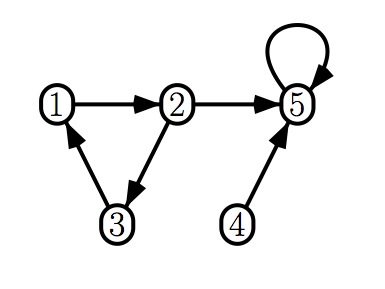
\includegraphics[scale=0.6]{images/1/RelationGraph}
\end{center}

\subsubsection{Seznamem seznamů}
Další způsob reprezentace pro uložení binární relace $R$ na množině $X$ (pro uložení binární relace v paměti počítače) je reprezentace seznamem seznamů. Tuto reprezentaci tvoří hlavní (spojový) seznam, ve kterém jsou uloženy všechny prvky množiny $X$. Z každého prcku $x \in X$ hlavního seznamu vede seznam obsahující právě ty $y \in X$, pro které platí $\langle x, y \rangle \in R$. Mějme relaci $R = \{\langle a, b\rangle,\langle a, d\rangle,\langle c, a\rangle,\langle b, d\rangle\}$ na množině $X = \{a,b,c,d\}$ potom reprezentace seznamem seznamů vypadá následovně.

\begin{center}
	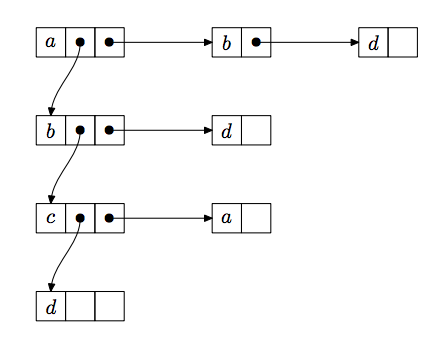
\includegraphics[scale=0.6]{images/1/RelationList}
\end{center}


\end{document}
